
Linear Meld (LM) is a \emph{forward chaining} logic programming language in the style of Datalog~\cite{Ullman:1990:PDK:533142}. The program is defined as a \emph{database of facts} and a set of \emph{derivation rules}.
Initially, we populate the database with the program's axioms and then determine which derivation rules can be applied by using the current database. Once a rule is applied, we derive new facts, which are then added to the database.
If a rule uses linear facts, they are consumed and thus deleted from the database.
The program stops when we reach \emph{quiescence}, that is, when we can no longer
apply any derivation rules.

The database of facts can be seen as a graph data structure where each node contains a
fraction of the database.
Because the derivation rules can only manipulate facts belonging to
a node, we are able to perform independent rule derivations at the node level, thus
exploiting concurrency in the program.

\section{A taste of LM}

\begin{figure}[h!]
\small\begin{Verbatim}[numbers=left]
type route edge(node, node).
type linear message(node, int, list node).
type linear processed(node, int).

!edge(A, B),
message(A, Content, [B | L]),
processed(A, N)
   -o message(B, Content, L),
      processed(A, N + 1).

message(A, Content, []),
processed(A, N)
   -o processed(A, N + 1).

!edge(@1, @2). !edge(@2, @3). !edge(@3, @4). !edge(@1, @3).
processed(A, 0).
message(@1, 42, [@3, @4]).
\end{Verbatim}
\caption{Message program.}
  \label{code:message}
\end{figure}

In order to show how LM can be used, we present some LM program examples.
Our first example shown in Fig.~\ref{code:message} is a message routing program
that simulates message transmission through a network of nodes.
We first declare all the predicates (lines 1-3), which represent the kinds of facts we are going to
use. Predicate \texttt{edge/2} is a non \texttt{linear} (persistent) while all the other predicates are linear.
Note that \texttt{edge/2} is also a \texttt{route} predicate, where the \texttt{edge} facts are used
for communication between nodes. The second argument of the \texttt{message/2} predicate is the message content
while the third argument is the route list.
Next, we declare the program rules (lines 5-13),
followed by the program axioms (lines 14-17).

The first rule (lines 5-9) grabs the next node in the route list (third argument of \texttt{message}) and
ensures that a communication edge exists (through \texttt{edge(A,~B)}). We increase the number of
processed messages by consuming \texttt{processed(A,~N)} and deriving \texttt{processed(A,~N~+~1)}.
When the route list is empty, the message has reached its destination and thus it is consumed
(rule in lines 11-13).
Note that we only need to send one message since there is only one \texttt{message} axiom (line 17).

In Fig.~\ref{fig:message_trace} we present an execution trace of the message routing program.
The database is represented as a graph structure where the edges represent the \texttt{edge}
axioms. We also use the first argument of each fact to partition the database.
In Fig.~\ref{fig:message_trace}~(a) the database is initialized with the program's axioms. Note that
the \texttt{message} fact is instantiated at node $@1$. After applying rule 1, we get the database represented
in Fig.~\ref{fig:message_trace}~(b), where the message has been derived at node $@3$. After applying rule 1 again,
the message is then routed to node $@4$ (Fig.~\ref{fig:message_trace}~(c)) where it will be consumed (Fig.~\ref{fig:message_trace}~(d)).

\begin{figure}[h]
        \centering
        \begin{subfigure}[b]{0.5\textwidth}
                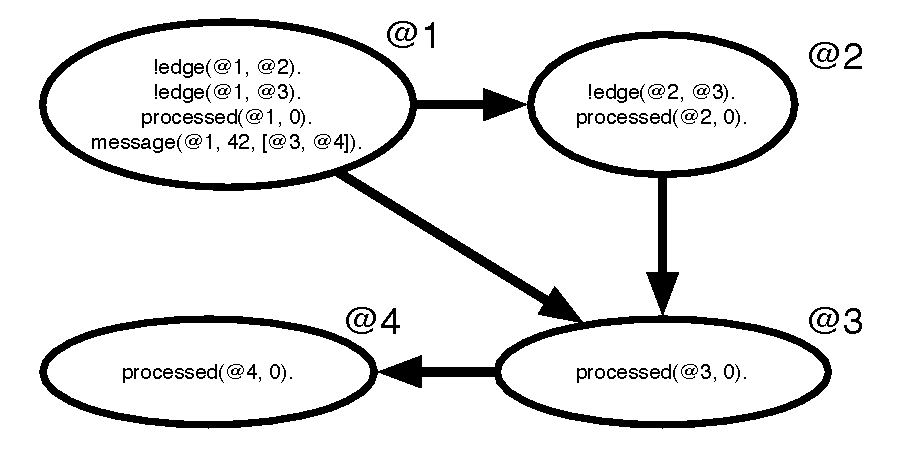
\includegraphics[width=\textwidth]{message_trace1}
                \caption{Initial database.}
                \label{fig:message_trace1}
        \end{subfigure}%
        ~
        \begin{subfigure}[b]{0.5\textwidth}
                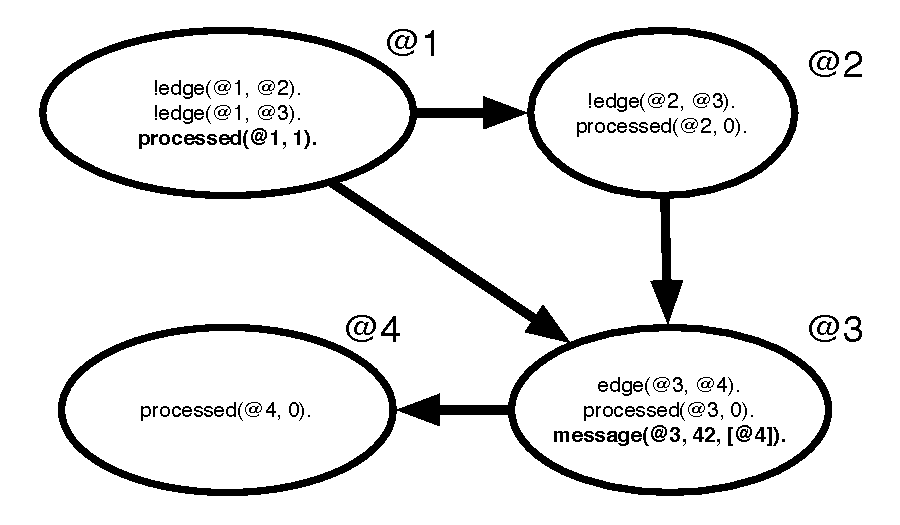
\includegraphics[width=\textwidth]{message_trace2}
                \caption{After applying rule 1 at node $@1$.}
                \label{fig:message_trace2}
        \end{subfigure}\\
        \begin{subfigure}[b]{0.5\textwidth}
                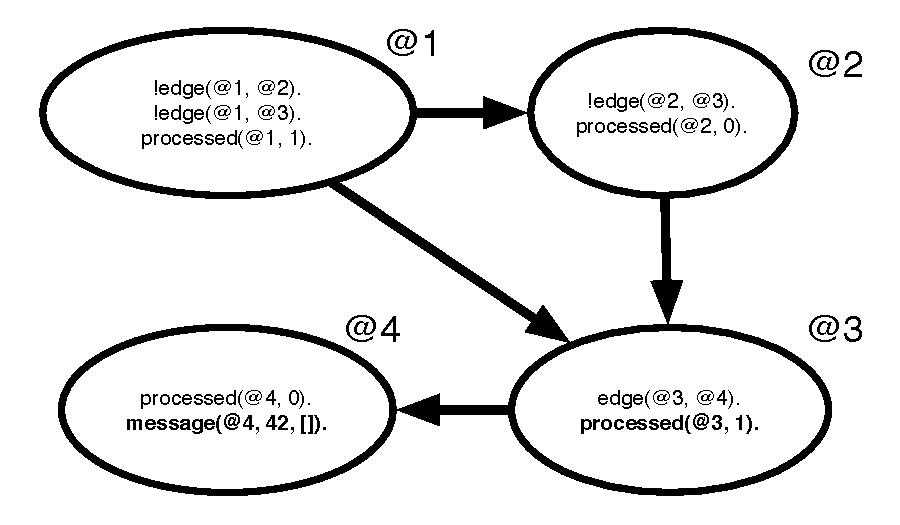
\includegraphics[width=\textwidth]{message_trace3}
                \caption{After applying rule 1 at node $@3$.}
                \label{fig:message_trace3}
        \end{subfigure}%
        ~
        \begin{subfigure}[b]{0.5\textwidth}
                  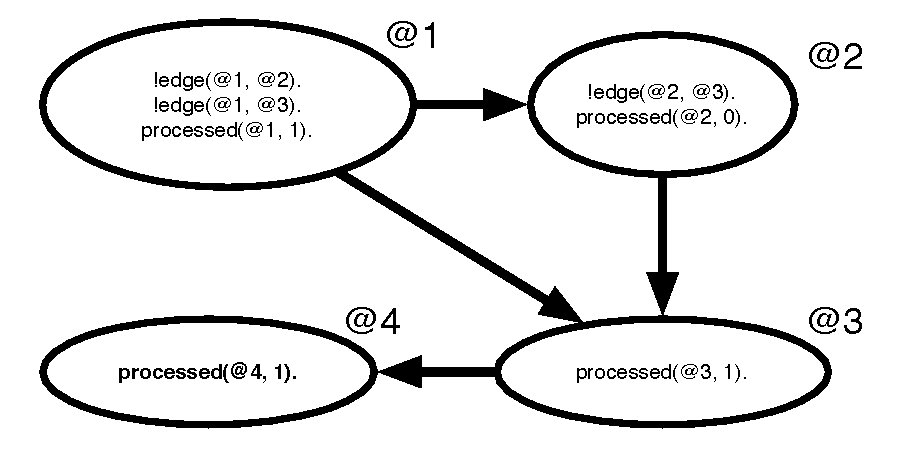
\includegraphics[width=\textwidth]{message_trace4}
                  \caption{After applying rule 2 (nodes $@4$).}
                  \label{fig:message_trace4}
          \end{subfigure}
        \caption{An execution trace for the message program.}\label{fig:message_trace}
\end{figure}

\begin{figure}[h!]
\small\begin{Verbatim}[numbers=left]
type route edge(node, node).
type linear visit(node).
type linear unvisited(node).
type linear visited(node).

// the program rules
visit(A), unvisited(A) -o
   visited(A), {B | !edge(A, B) | visit(B)}.

visit(A), visited(A) -o visited(A).

// axioms: the input data
!edge(@1, @2). !edge(@2, @3). !edge(@1, @4). !edge(@2, @4).
unvisited(@1). unvisited(@2). unvisited(@3). unvisited(@4).

visit(@1).
\end{Verbatim}
  \caption{Visit program.}
  \label{code:visit}
\end{figure}
\normalsize

Figure~\ref{code:visit} presents another complete LM program that, for a given graph
of nodes, performs a visit to all nodes reachable from node $@1$.
The first rule of the program (lines 7-8) is fired when a node has a \texttt{visit} and a \texttt{unvisited} fact. When fired, we first derive \texttt{visited} to mark node as \textit{visited} and use a
\emph{comprehension} construct to go through all the edge facts and derive \texttt{visit} for every
one of them. This forces those nodes to be visited also. The second rule (line 10) is fired when the
node is already visited more than once: we keep the \texttt{visited} fact and delete \texttt{visit}.
Node $@1$ starts with the \texttt{visit(@1)} fact (line 16).

Fig.~\ref{fig:exec_trace} shows a possible execution trace for the visit program.
After applying the first rule at node $@1$ we get the database in Fig~\ref{fig:exec_trace}~(b).
Note that node $@1$ is now \texttt{visited} and nodes $@2$
and $@4$ now have the fact \texttt{visit}. At this point we could either apply rule 1 at
node $@2$ or at node $@4$. For this specific trace, we apply the rule at node $@2$, resulting
in Fig.~\ref{fig:exec_trace}~(c). Node $@4$ now has 2 \texttt{visit} facts, thus
we can apply rule 1 followed by rule 2, therefore consuming both \texttt{visit} facts
and deriving \texttt{visited}. In addition, we can also apply rule 1 at node $@3$ to
reach the state of Fig.~\ref{fig:exec_trace}~(d).

\begin{figure}[h]
        \centering
        \begin{subfigure}[b]{0.5\textwidth}
                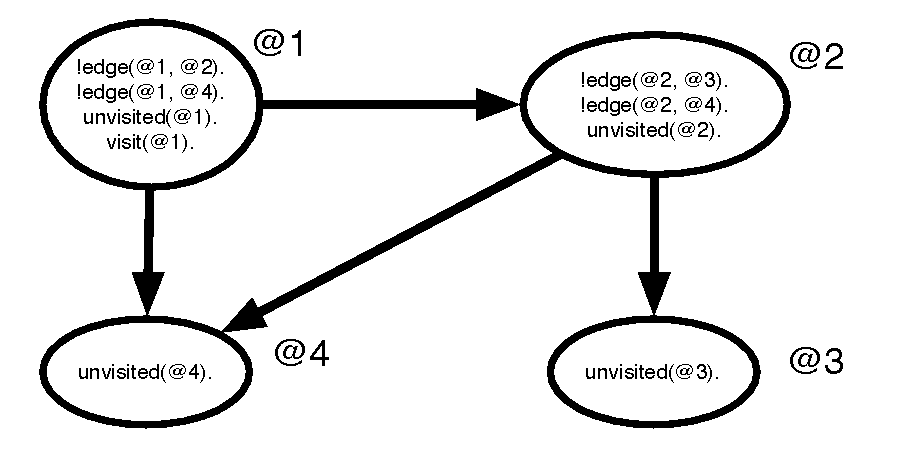
\includegraphics[width=\textwidth]{execution_trace1}
                \caption{Initial database.}
                \label{fig:exec_trace1}
        \end{subfigure}%
        ~ %add desired spacing between images, e. g. ~, \quad, \qquad etc.
          %(or a blank line to force the subfigure onto a new line)
        \begin{subfigure}[b]{0.5\textwidth}
                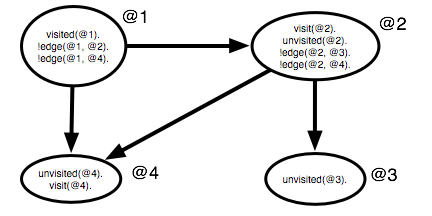
\includegraphics[width=\textwidth]{execution_trace2}
                \caption{After applying rule 1 at node $@1$.}
                \label{fig:exec_trace2}
        \end{subfigure}\\
        \begin{subfigure}[b]{0.5\textwidth}
                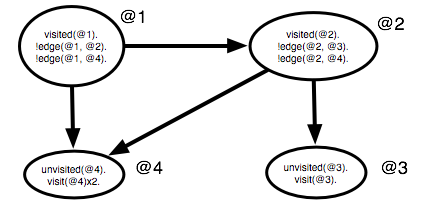
\includegraphics[width=\textwidth]{execution_trace3}
                \caption{After applying rule 1 at node $@2$.}
                \label{fig:exec_trace3}
        \end{subfigure}%
        ~ %add desired spacing between images, e. g. ~, \quad, \qquad etc.
         %(or a blank line to force the subfigure onto a new line)
        \begin{subfigure}[b]{0.5\textwidth}
                  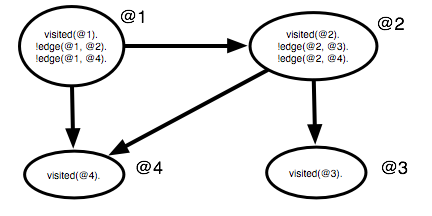
\includegraphics[width=\textwidth]{execution_trace4}
                  \caption{After applying rule 1 and 2 (nodes $@3$, $@4$).}
                  \label{fig:exec_trace4}
          \end{subfigure}
        \caption{A possible execution trace for the visit program.}\label{fig:exec_trace}
\end{figure}

Note that every node is now \texttt{visited}. It is easy to prove that if the graph is
connected, then all the nodes will be \texttt{visited}, regardless the order in which we
apply the rules.

\section{Syntax}

\renewcommand{\arraystretch}{1.5}

\begin{table}[h]
   \centering
\begin{tabular}{ l l c l }
  Linear Facts & $L$ & $::=$ & $l(\hat{x})$\\
  Persistent Facts & $P$ & $::=$ & $\bang p(\hat{x})$\\
  Constraints & $C$ & $::=$ & $c(\hat{x})$ \\
  Action Facts & $A$ & $::=$ & $a(\hat{x})$\\
  Sensing Facts & $S$ & $::=$ & $s(\hat{x})$\\
  Body Expressions & $BE$ & $::=$ & $L \; | \; P \; | \; C \; | \; BE, BE \; | \; \forall_{\widehat{x}}. BE \; | \; \exists_{\widehat{x}}. BE \; | \; 1$\\
  Comprehensions & $CE$ & $::=$ & $\{ \; \widehat{x} \; | \; BE \; | \; HE \; \}$ \\
  Aggregates & $AE$ & $::=$ & $[\;\m{aop} \Rightarrow y \; | \; \widehat{x} \; | \; BE \; | \; HE_1 \; | \; HE_2 \;]$ \\
  Exists constructs & $EE$ & $::=$ & $exists \; \widehat{x}. (HE)$ \\
  Head Expressions & $HE$ & $::=$ & $A \; | \; L \; | \; P \; | \; HE, HE \; | \; EE \; | \; CE \; | \; AE \; | \; 1$\\
  Rules & $R$ & $::=$ & $BE \lolli HE \; | \; [\; \m{sop} \Rightarrow y \; | \; BE \;] \lolli HE$ \\
  Set Of Rules & $\Sigma$ & $::=$ & $\cdot \; | \; \Sigma, R$\\
  Known Linear Facts & $\Delta$ & $::=$ & $\cdot \; | \; \Delta, l(\hat{t})$ \\
  Known Persistent Facts & $\Gamma$ & $::=$ & $\cdot \; | \; \Gamma, \bang p(\hat{t})$ \\
  Database & $D$ & $::=$ & $\Gamma; \Delta$ \\
\end{tabular}
\caption{Abstract syntax of LM.}\label{tbl:ast}
\end{table}

\renewcommand{\arraystretch}{1.0}

Table~\ref{tbl:ast} shows the abstract syntax for rules in LM.
A LM program consists of a set of derivation rules ($\Sigma$) and a database ($D$).
Each derivation rule can be written as $BE \lolli HE$ where $BE$ is the body of a rule and
$HE$ is the head. Rules without bodies are allowed in LM and they are called \textit{axioms} (lines 13-16 in Fig.~\ref{code:visit}). Rules without heads are also allowed.

The body of the rule ($BE$) contains \emph{fact expressions} ($L$ and $P$) and
constraints ($C$). Fact expressions are template facts that instantiate variables
(from facts in the database)
such as \texttt{visit(A)} in line 10 in Fig.~\ref{code:visit}. Variables can be used again in the body for matching and
also in the head when instantiating facts. Constraints are boolean expressions that must
be true in order for the rule to be fired. Constraints use variables from fact expressions and are built using a small functional language that includes mathematical operations, boolean operations, external functions and literal values.

The head of a rule ($HE$) contains \emph{fact templates} ($L$ and $P$) which are uninstantiated facts and will derive new facts. The head can also have \emph{exist constructs} ($EE$), \emph{comprehensions} ($CE$) and \emph{aggregates} ($AE$). All those constructs
may use all the variables instantiated in the body.

\subsection{Predicates and Facts}

Each fact is an association between a \emph{predicate} and a tuple of values. A predicate is a pair with a name and a tuple of types (the argument types). LM rules are type-checked using the predicate declarations in the header of the program. LM has a simple type system that includes the following simples types: \emph{node}, \emph{int}, \emph{float}, \emph{string}, \emph{bool}. Recursive types such as \emph{list X} and \emph{pair X; Y} are
also allowed.

\subsection{Comprehensions}

Sometimes we need to consume a linear fact and then immediately generate several facts depending on
the contents of the database. To solve this particular need, we created the concept of comprehensions, which are
sub-rules that are applied with all possible combinations of facts from the database. In a comprehension $\{ \; \widehat{x} \; | \; BE \; | \; HE \; \}$,
$\widehat{x}$ is a list of variables, $BE$ is the body of the comprehension and $HE$ is the head.
The body $BE$ is used to generate all possible combinations for the head $HE$, according to the facts
in the database.
We have already seen an example of comprehensions in the visit program (Fig.~\ref{code:visit} line 8).
Here, we match \texttt{!edge(A, B)} using all the combinations
available in the database and for each combination we derive \texttt{visit(B)}.

\subsection{Aggregates}

Another useful feature in logic programs is the ability to reduce several facts into a single fact.
In LM we have aggregates ($AE$), a special kind of sub-rule that works very similarly to comprehensions.
In the abstract syntax $[\;\m{aop} \Rightarrow y \; | \; \widehat{x} \; | \; BE \; | \; HE_1 \; |
\; HE_2 \;]$, $\m{aop}$ is the aggregate operation, $\widehat{x}$ is the list of variables
introduced in $BE$, $HE_1$ and $HE_2$ and $y$ is the variable in the body
$BE$ that represents the values to be aggregated using $\m{aop}$. Like comprehensions,
we use $\widehat{x}$ to try all the combinations of $BE$, but, in addition to deriving $HE_1$ for each combination,
we aggregate the values represented by $y$ and derive $HE_2$ only once using $y$.

To better understand aggregates, let's consider a database with the following facts and a rule:

\begin{Verbatim}
price(@1, 3).
price(@1, 4).
price(@1, 5).
count-prices(@1).
count-prices(A) -o [:sum => P | price(A, P) | | total(A, P)].
\end{Verbatim}

By applying the rule, we consume \texttt{count-prices(@1)} and
derive the aggregate which consumes all the \texttt{price(@1, P)} facts.
These are summed and \texttt{total(@1,~12)} is derived since \texttt{P~=~12}.  
LM provides several aggregate operations, including the minimum, maximum, sum, and count.

\subsection{Selectors}

When a rule body is instantiated using facts from the database, facts are picked
non-deterministically. While our system uses an implementation dependent order for
efficiency reasons, sometimes it is important to sort facts by one of the arguments
because linearity imposes commitment during rule derivation. The abstract syntax for
this construct is $[\; \m{sop} \Rightarrow y \; | \; BE \;] \lolli HE$, where
$\m{sop}$ is the selection operation and $y$ is the variable in the body $BE$ that
represents the value to be selected according to $\m{sop}$.
An example using concrete syntax is as follows:

\begin{Verbatim}
[:min => W | !edge(A, B), weight(A, B, W)]
                              -o edge-picked(A, B, W).
\end{Verbatim}

In this case, we will order the \texttt{weight} facts by $W$ in ascending order and then try
to match them. Other operations available are \texttt{max} and \texttt{random} (to force no pre-defined order at the
implementation level).

\subsection{Exists Constructs}

Exist constructs ($EE$) are based on the linear logic construct of the same name and are used to create new node addresses. We can use the new address to instantiate new facts for the new node.  
The following example illustrates the use of the exists construct, where we derive
\texttt{perform-work} at a new node \texttt{B}.

\begin{Verbatim}
   do-work(A, W) -o exists B. (perform-work(B, W)).
\end{Verbatim}

\section{Types of Facts}

Beyond the distinction between linear and persistent facts, LM further classifies facts
into 4 categories: \emph{computation} facts, \emph{structural} facts, \emph{sensing} facts
and \emph{action} facts. Predicates are also classified accordingly.

Computation facts are regular facts used to represent the program state. In the initial
example in Fig.~\ref{code:visit}, \texttt{visit/1}, \texttt{visited/1} and \texttt{unvisited/1}
are all computation facts.

Structural facts describe information about the connections between the nodes in the graph.
In the example of Fig.~\ref{code:visit}, \texttt{edge/2} facts are structural since the
corresponding \texttt{edge/2} predicate is
marked as a \texttt{route} predicate. Note that structural facts can also be seen as
computation facts since they are heavily used in the program algorithm.

Sensing facts are facts about the current state of the runtime system, such as the placement
of nodes in the CPU and scheduling information. In the original Meld, sensing facts
were used to get information about the outside world, like temperature, touch data,
neighborhood status, etc.

Action facts are linear facts which are consumed when the corresponding action is performed.
In the original Meld, they were used to make the robots perform actions in the outside world.
For LM we use them to change information about the program state
in the user interface. For example, when we want to change the color of nodes or the label
of edges, we just derive a new action fact and the action is performed in the interface.
A more important use of action facts is to change the order in which nodes
are evaluated in the runtime system. It is possible to give hints to the virtual
machine in order to prioritize the computation of some nodes.

With sensing facts and action facts, we can write \emph{meta-rules} that will sense the
state of the runtime system and then apply decisions in order to improve execution speed.
In some situations, this set of rules can be added to the program without any modifications
to the original rules.

\section{Operational Semantics}

The first argument of every predicate must be typed as a \emph{node}.
For distribution and data partitioning purposes, derivation rules are constrained by the expressions that can be written in the body.
The body of every rule can only refer to facts in the same node.
However, the expressions in the head may refer to other nodes, as long as those nodes are instantiated in the body of the rule.
The database of the program can then be partitioned by the first argument of each fact. 
We drew some inspiration from the Linda system~\cite{1663305}, where the tuple space contains the data and is used by the processors
to communicate and do computation.
This differs from imperative languages, since in those languages data and computation are two separate entities.

The execution is performed at the node level and can happen non-deterministically (i.e., any node can
be picked to run). This means that the programmer cannot expect
that facts coming from other nodes will be considered as a whole or partially since the process is non-deterministic.
Under these restrictions, computation can then be parallelized by processing many nodes concurrently.

Each rule in LM has a defined priority that is inferred from its position in the source file.
Rules at the beginning of the file have higher priority. At the node level, we consider all
the new facts that have been not consider before to create a set of \emph{candidate rules}.
The set of candidate rules is then applied (by priority) and updated as new facts are derived or consumed.
Section~\ref{sec:core_engine} gives details in how our implementation manages the set of candidate rules.

\section{Programs}

In this section, we present several LM programs in order to show that they tend to be concise and
easy to write. We also want to make clear how the language facilities can be used to solve more
complicated algorithms, including the quick-sort algorithm that at the first glance does not seem
to fit the graph based paradigm of LM.

\subsection{Bipartiteness Checking}

The problem of checking if a graph is bipartite can be seen as a 2-color graph coloring problem.
The code for this algorithm is shown in Fig.~\ref{code:bichecking}. All nodes in the graph
start as \texttt{unchecked}, because they do not have a color yet. The axiom \texttt{visit(@1, 1)} is
instantiated at node \texttt{@1} (line 9) in order to color this node with color 1.

If a node is \texttt{unchecked} and needs to be marked with a color \texttt{P} then the rule in
lines 11-12 is applied. We consume the \texttt{unchecked} fact and derive a \texttt{checked(A, P)}
to effectively color the node with \texttt{P}. We also derive \texttt{visit(B, next(P))} in
neighbor nodes to color them with the other color.

The coloring can fail if a node is already colored with a color \texttt{P} and needs to be colored
with a different color (line 15) or if it has already failed (line 16).

\begin{figure}[h!]
\small\begin{Verbatim}[numbers=left]
type route edge(node, node).
type linear visit(node, int).
type linear unchecked(node).
type linear checked(node, int).
type linear fail(node).

fun next(int X) : int = if X <> 1 then 1 else 2 end.

visit(@1, 1).

visit(A, P), unchecked(A)
   -o {B | !edge(A, B) | visit(B, next(P))}, checked(A, P).

visit(A, P), checked(A, P) -o checked(A, P).
visit(A, P1), checked(A, P2), P1 <> P2 -o fail(A).
visit(A, P), fail(A) -o fail(A).
\end{Verbatim}
  \caption{Bipartiteness Checking program.}
  \label{code:bichecking}
\end{figure}
\normalsize

\subsection{N Queens}

The N queens~\cite{8queens} puzzle is the problem of placing N chess queens on an NxN chessboard so
that no pair of two queens attack each other. The specific challenge of finding all the distinct
solutions to this problem is a good benchmark in designing parallel algorithms.

First, we consider each square of the chessboard as a node
that can communicate with the adjacent left, right and bottom squares, but not top square.
The states are represented as a list of integers, where each integer is the column number where
the queen was placed. For example $[2, 0]$ means that a queen is placed in square $(0, 0)$ and another in square $(1, 2)$.

An empty state is instantiated in the top-left node and is then propagated to all nodes in the same row.
Every node will then check if a queen can be placed on such square. If true, each node will send at most
two new states to the row below, one to the first non-diagonal column to the left and another to the column
in the right.
Recursively, when a node receives a new state, it will (i) send the state to the left
or to the right and (ii) try to place the queen in its square. With this method,
all states will be computed since we have facts for each valid state
at that point. When a suare cannot place a queen, that state is deleted.
When the program ends, all valid states will be placed in the bottom row.

We find our solution very elegant, since it can be easily executed in parallel and is an uncommon
approach to this problem.

\begin{comment}
\begin{figure}[h!]
\small\begin{Verbatim}[numbers=left]
type left(node, node).
type right(node, node).
type down(node, node).
type coord(node, int, int).
type linear propagate-left(node, list node, list int).
type linear propagate-right(node, list node, list int).
type linear receive-down(node, list node, list int).
type linear test-and-send-down(node, list node, list int).
type linear test-y(node, int, list int, list node, list int).
type linear test-diag-left(node, int, int, list int, list node, list int).
type linear test-diag-right(node, int, int, list int, list node, list int).
type linear send-down(node, list node, list int).
type linear final-state(node, list node, list int).

const size = 11.

receive-down(@0, [], []).

receive-down(A, Nodes, Coords)
   -o {R | !right(A, R), R <> A | propagate-right(R, Nodes, Coords)},
      {L | !left(A, L), L <> A | propagate-left(L, Nodes, Coords)},
      test-and-send-down(A, Nodes, Coords).

propagate-left(A, Nodes, Coords)
   -o {L | !left(A, L), L <> A | propagate-left(L, Nodes, Coords)},
      test-and-send-down(A, Nodes, Coords).

propagate-right(A, Nodes, Coords)
   -o {R | !right(A, R), R <> A | propagate-right(R, Nodes, Coords)},
      test-and-send-down(A, Nodes, Coords).

test-and-send-down(A, Nodes, Coords),
!coord(A, X, Y)
   -o test-y(A, Y, Coords, Nodes, Coords).

test-y(A, Y, [], Nodes, Coords), !coord(A, OX, OY) -o test-diag-left(A, OX - 1, OY - 1, Coords, Nodes, Coords).
test-y(A, Y, [X, Y1 | RestCoords], Nodes, Coords), Y = Y1 -o 1. // fail
test-y(A, Y, [X, Y1 | RestCoords], Nodes, Coords), Y <> Y1 -o test-y(A, Y, RestCoords, Nodes, Coords).

test-diag-left(A, X, Y, _, Nodes, Coords),
X < 0 || Y < 0,
!coord(A, OX, OY)
   -o test-diag-right(A, OX - 1, OY + 1, Coords, Nodes, Coords).

test-diag-left(A, X, Y, [X1, Y1 | RestCoords], Nodes, Coords),
X = X1, Y = Y1
   -o 1. // fail

test-diag-left(A, X, Y, [X1, Y1 | RestCoords], Nodes, Coords),
X <> X1 || Y <> Y1
   -o test-diag-left(A, X - 1, Y - 1, RestCoords, Nodes, Coords).

test-diag-right(A, X, Y, [], Nodes, Coords),
X < 0 || Y >= size,
!coord(A, OX, OY)
   -o send-down(A, [A | Nodes], [OX, OY | Coords]).

test-diag-right(A, X, Y, [X1, Y1 | RestCoords], Nodes, Coords),
X = X1, Y = Y1
   -o 1. // fail

test-diag-right(A, X, Y, [X1, Y1 | RestCoords], Nodes, Coords),
X <> X1 || Y <> Y1
   -o test-diag-right(A, X - 1, Y + 1, RestCoords, Nodes, Coords).

send-down(A, Nodes, Coords),
!down(A, A)
   -o final-state(A, Nodes, Coords).
   
send-down(A, Nodes, Coords),
!down(A, B),
A <> B
   -o receive-down(B, Nodes, Coords).
\end{Verbatim}
  \caption{Visit program.}
  \label{code:visit}
\end{figure}
\normalsize
\end{comment}

\subsection{Quick-Sort}

The quick-sort algorithm is a divide and conquer sorting algorithm that works by splitting
a list of items into two sublists and then recursively sorting the two sublists.
To split the list, we pick a pivot element and put the items that are smaller than the pivot
into the first sublist and items greater than the pivot into the second list.

The quick-sort algorithm is interesting because it does not map immediately to the graph-based
model of LM. Our approach considers that the program starts with a single node where
the initial list is located. Then we split the list as usual and create two nodes
that will recursively sort the sublists. Interestingly, this will create a tree
that will look similar to a call tree in a functional language.

Fig.~\ref{code:quicksort} presents the code for the quick-sort algorithm in LM.
For each sublist to sort, we start with a \texttt{down} fact that must be (eventually)
transformed into an \texttt{up} fact, where the sublist in the \texttt{up} fact is sorted.
In line 11 we start with the initial list at node \texttt{@0}. Lines 13-16 will immediately
sort the list when the number of items is very small. Otherwise, we apply the rule in line 17.
\texttt{buildpivot} will first split the list using the pivot \texttt{X} using rules in
lines 23-26. When there is nothing more to split, we apply the rule in lines 19-21
that uses an exist construct to create nodes \texttt{B} and \texttt{C}. The sublists
are then sent to these nodes using \texttt{down} facts. Note, however, that we also
derive \texttt{back} facts, that will be used to send the sorted list back using the rule
in line 40.

When the sublists are finally sorted, we get two \texttt{sorted} facts that will match
against \texttt{waitpivot} in the rule located in lines 28-31. The sorted sublists
are appended and then an \texttt{up} fact is finally derived (line 37).

\begin{figure}[h!]
\small\begin{Verbatim}[numbers=left]
type route back(node, node).
type linear down(node, list int).
type linear up(node, list int).
type linear sorted(node, node, list int).
type linear buildpivot(node, list int, int, list int, list int).
type linear waitpivot(node, node, node, int).
type linear append(node, list int, list int).
type linear reverse(node, list int, list int, list int).
type linear reverse2(node, list int, list int).

down(@0, tosort).

down(A, []) -o up(A, []).
down(A, [X]) -o up(A, [X]).
down(A, [X, Y]), X < Y -o up(A, [X, Y]).
down(A, [X, Y]), X >= Y -o up(A, [Y, X]).
down(A, [X | L]) -o buildpivot(A, L, X, [], []).

buildpivot(A, [], X, Smaller, Greater)
   -o exists B, C. (back(B, A), down(B, Smaller),
            back(C, A), down(C, Greater), waitpivot(A, B, C, X)).

buildpivot(A, [Y | L], X, Smaller, Greater), Y <= X
   -o buildpivot(A, L, X, [Y | Smaller], Greater).
buildpivot(A, [Y | L], X, Smaller, Greater), Y > X
   -o buildpivot(A, L, X, Smaller, [Y | Greater]).
   
waitpivot(A, NodeSmaller, NodeGreater, Pivot),
sorted(A, NodeSmaller, Smaller),
sorted(A, NodeGreater, Greater)
   -o append(A, Smaller, [Pivot | Greater]).

append(A, L1, L2) -o reverse(A, L1, L2, []).

reverse(A, [], L2, L3) -o reverse2(A, L3, L2).
reverse(A, [X | L], L2, L3) -o reverse(A, L, L2, [X | L3]).
reverse2(A, [], Result) -o up(A, Result).
reverse2(A, [X | L1], L2) -o reverse2(A, L1, [X | L2]).

up(A, L), back(A, B) -o sorted(B, A, L).
\end{Verbatim}
  \caption{Quick-Sort program.}
  \label{code:quicksort}
\end{figure}
\normalsize


\section{Summary}

In this chapter we gave an overview of the LM language, including its syntax and operational semantics.
We also explained how to write programs using all the facilities provided by LM, including
linear facts and comprehensions. Since LM uses implicit parallelism, programs can be run in parallel
in multicore architectures without any modification.
